\section{Le testeur sous pointes et ADWin}
\begin{figure}[h]
    \begin{center}
        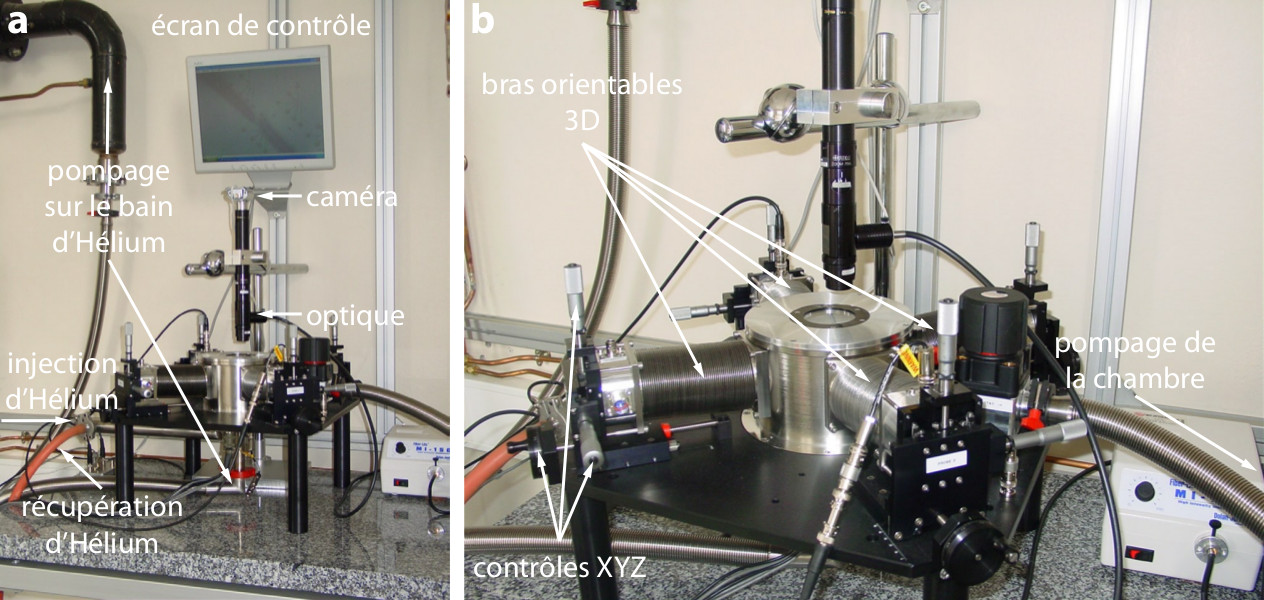
\includegraphics[width=250px]{Images/ADWin_avec_legendes}
        \caption{Le Testeur sous Pointes}
        \label{fig:}
        Photo disponible à \url{https://tel.archives-ouvertes.fr/tel-00456601v2/document}
    \end{center}
\end{figure}
Pour réaliser l'électromigration, on a besoin du testeur sous pointes qui, grâce à ses quatre bras orientables supportant les pointes, permet d'imposer une rampe de tension et de mesurer simultanément la conductance. Le testeur sous pointe possède un accès optique permettant de connecter rapidement les échantillons et de les refroidir à 4,2K. Notons que le contact est moins bon qu'avec des microsoudures. 
\begin{figure}[h]
    \begin{center}
        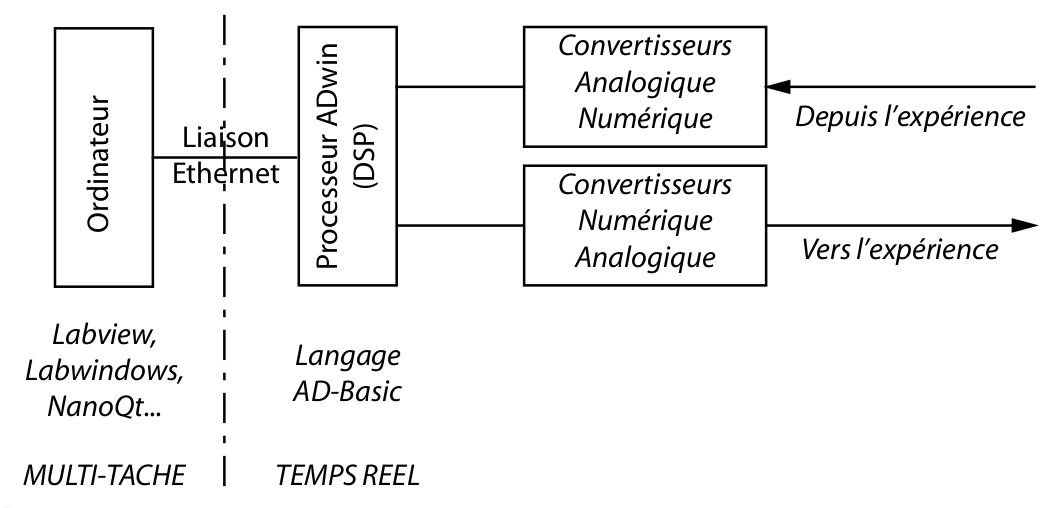
\includegraphics[width=250px]{Images/ADWin_schema}
        \caption{Schéma de fonctionnement d'ADWin}
        \label{fig:}
        Schéma disponible à \url{https://tel.archives-ouvertes.fr/tel-00456601v2/document}
    \end{center}
\end{figure}

On doit disposer d'une électronique de mesure en temps réel et d'une détection synchrone : c'est le rôle d'ADWin.

La première partie constituant ADWin est l'ordinateur permettant le stockage des données et l'interface graphique. Vient ensuite le processeur propre à ADWin qui garantit la répétition de suites d'instructions toutes les 3,3ns. Ceci est une nécessité car un OS (multitâche) ne pourrait garantir une base de temps inférieur à 10ms et compromettrait le résultat de l'électromigration. Enfin les convertisseurs génèrent et reçoivent les signaux expérimentaux.

Un des autres avantages d'ADWin est la diminution du bruit. En incrémentant bit par bit des rampes de mesures (tension, courant) et grâce à la très petite base de temps du système on peut balayer des plages entière de tension, courant, charges en des temps très faible et obtenir une très bonne précision.

\section{Le fullerène}
Les fullerènes sont des molécules composées de carbone d'un nanomètre de diamètre. Leur découverte en 1985 a donné lieu au prix Nobel de chimie 1996 et à toute une nouvelle classe de matériau massique. Le fullerène utilisé est le C$_{60}$, une molécule très simple de la forme d'un ballon de football.

\begin{figure}[h]
    \begin{center}
        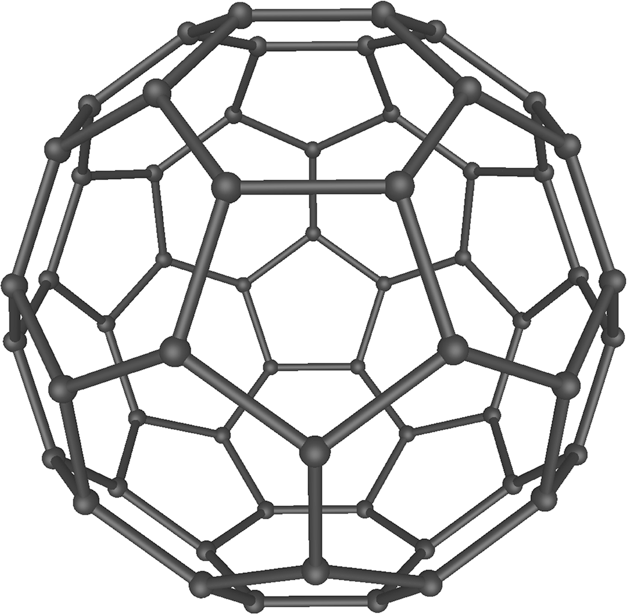
\includegraphics[width=100px]{Images/C60.png}
        \caption{Structure de la molécule de Fullerène}
        \label{fig:}
    \end{center}
\end{figure}

On dépose le fullerène C$_{60}$ avant l'étape d'électromigration et on espère qu'une molécule tombe dans le gap créé sur le nanofil d'or. La probabilité d'occurrence est plus importante que si l'on essaye de déposer une molécule dans un gap préexistant. On essaye d'avoir des molécules uniques de C$_{60}$ plutôt que des agrégats car la molécule unique présente une énergie de charge plus importante et un couplage à l'environnement moins fort gage de stabilité. Une dilution dans le toluène permet de caractériser si une solution est composée de molécules uniques (couleur jaune) ou d'agrégats (couleur violette).


\section{L'électromigration}
L'électromigration est un phénomène bien connu en microélectronique. Il s'agit d'un transport de matière observé dans les métaux traversés par de fortes densités de courant ; c'est une cause d'endommagement des interconnexions métalliques et donc de fiabilité dans les circuits intégrés\cite{8}. Ce phénomène est néfaste pour la microélectronique "classique", mais son utilisation est très intéressante pour la réalisation de transistors à molécule unique. En effet il faut que la molécule soit reliée à un dispositif métallique macroscopique et donc que les électrodes (source-drain) soient séparées d'une distance nanométrique proche de la taille de la molécule ; ce qui est impossible par des méthodes de nanofabrication limitées à environ 10nm de résolution, alors qu'une résolution inférieure est possible grâce à l'électromigration\cite{9}.\\

Intéressons-nous maintenant à la description théorique de l'électromigration, "mise en mouvement des atomes par un métal causée par l'application d'un champ électrique". La force de transport peut être notée :
\[\vec{F}=e Z^* \vec{E}\]
où le terme $Z^*$ se décompose en deux parties, l'une modélisant l'effet du champ électrostatique, l'autre le "vent des électrons" qui transmettent leurs mouvements aux ions.
\[Z^* = Z_{\text{electrostatique}} + Z_{\text{vent}}\]
Dans les métaux c'est principalement le vent d'électrons qui est responsable du transport, ainsi le transport de matière a lieu dans le sens de circulation des électrons\cite{10}.\\

Il faut maintenant pouvoir suivre l'électromigration pour pouvoir réaliser un nanogap, cela est possible grâce à une mesure en temps réel de la conductance (ou la résistance) à l'aide d'ADWin.\\

Au cours de l'électromigration, les propriétés de conduction vont évoluer et on peut distinguer deux régimes de conduction :
\begin{description}
    \item[Le régime diffusif,] lorsque le libre parcours moyen ($L_m \simeq 10nm$) est inférieur aux dimensions du nanofil
    \item[Le régime ballistique,] lorsque le libre parcours moyen est supérieur aux dimensions du nanofil
\end{description}

Or dans le cas du régime balistique, d'après la formule de Landauer Buttiker, la conductance est un multiple du quantum de conductance :
\[G = G_0 \sum_{n=1}^N T_n \quad \text{ où } \quad G_0 = \frac{2e^2}{h} = 77.5 \mu S\]
avec les T probabilités de transmission pour les N canaux de conduction.
\begin{figure}[h]
    \begin{center}
        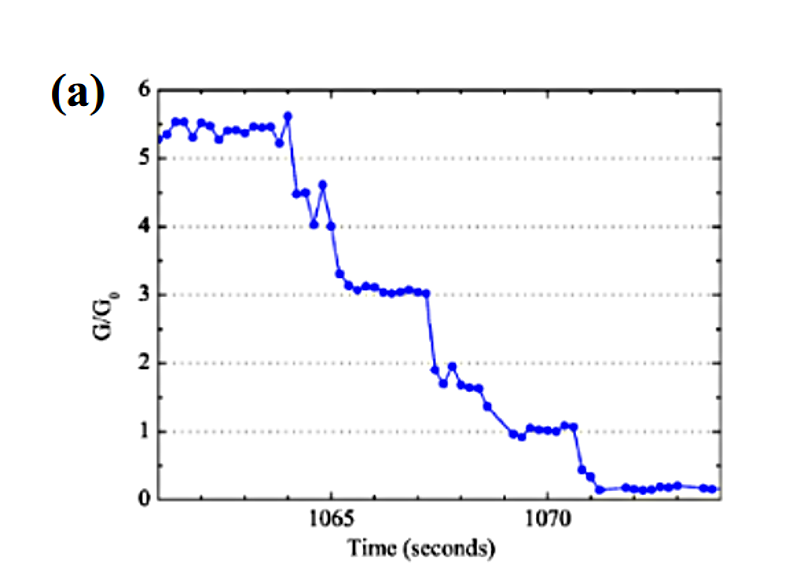
\includegraphics[width=250px]{Images/Electromigration_graphe}
        \caption{Variation de G en fonction du temps à la fin d’une électromigration (au moment de l’ouverture du nanogap).
On observe bien des paliers de conductance}
        Photo disponible à \url{https://tel.archives-ouvertes.fr/tel-00515127/document}
        \label{fig:}
    \end{center}
\end{figure}

On en déduit ainsi que si G<G${_0}$ ou R>R${_0}$, il n'y a plus de canaux de conduction et donc qu'on a crée un nanogap. Il suffit donc de stopper l'électromigration à cette limite de conductance dans un temps très court de l'ordre de la microseconde ce qui est possible grâce à l'électronique temps réel\cite{11}.

En réalité on stoppera plutôt notre expérience à R>2R${_0}$ qui expérimentalement assure de meilleurs résultats.

\section{Le blocage de Coulomb dans un transistor à électron unique}
\footnote{Cette partie s'inspire librement du cours de nanophysique de Monsieur Thierry Ouisse de 2A PNS ainsi que des aspects théoriques présentés dans \cite{3}, \cite{5}, \cite{10}, \cite{13} et \cite{15} qui présentent en détail le blocage de Coulomb.}
On considère un îlot quantique, placé entre 3 électrodes : le drain, la source et la grille. Le drain et la source sont séparés de l'îlot par des jonctions tunnels. On note V${_d}$, V${_s}$ et V${_g}$ respectivement les tensions de drain, source et grille. De plus, on note N le nombre d'électrons à l'intérieur de l'îlot. 
\begin{figure}[h]
    \begin{center}
        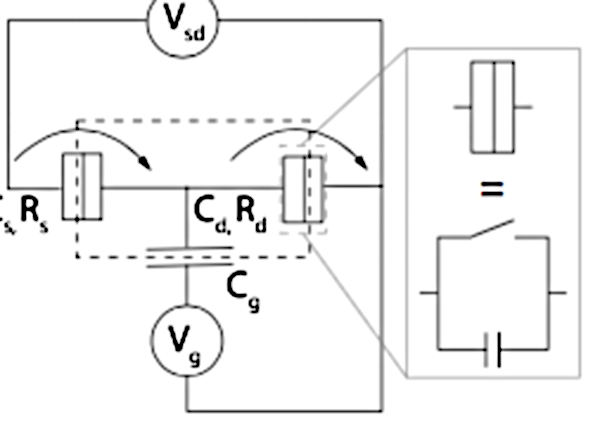
\includegraphics[width=250px]{Images/Blocage_Coulomb_Schema}
        \caption{Schéma équivalent du transistor}
        \label{fig:}
    \end{center}
\end{figure}

L'îlot possède donc une énergie électrostatique E${_c}$.

Ainsi, il va falloir apporter de l'énergie à un électron pour pouvoir le faire rentrer dans l'îlot Quantique. Si $V_{sd}>0$, il va être plus simple  d'injecter un électron dans l'îlot depuis la source plutôt que depuis le drain. Une fois l'électron apporté dans l'îlot, on modifie l'énergie à l'intérieur de l'îlot, ce qui va rendre plus difficile l'entrée d'un nouvel électron (on passe de N à N+1). Cette variation d'énergie doit être négative si l'on veut continuer à faire rentrer des électrons:
\[\Delta E = \frac{e}{C_1 + C_2 + C_G}\left((N + \frac{1}{2})e - C_G V_G - C_2 V_D\right)\]
ce qui donne la condition :
\[V_D > (N + \frac{1}{2})\frac{e}{C_2} - \frac{C_G}{C_2}V_G\]

De manière analogue, si $V_{sd}>0$, il va être plus facile de sortir un électron de l'îlot par le drain que par la source (on passe de N à N-1). On va cette fois ci avoir une variation d'énergie positive si l'on veut arrêter de faire rentrer des électrons dans l'îlot :
\[\Delta E = \frac{e}{C_1 + C_2 + C_G}\left(-(N + \frac{1}{2})e + C_G V_G - (C_1 + C_G) V_D\right)\]
(car il va être plus simple de rentrer un nouvel électron). Cette variation va donner la condition:
\[V_D > - (N + \frac{1}{2})\frac{e}{C_1 + C_G} + \frac{C_G}{C_1 + C_G}V_G\]

De même, on refait les mêmes raisonnements pour $V_{sd}<0$. Dans ce cas, il sera plus simple de rentrer un électron dans l'îlot à partir du drain et d'en sortir un à partir de la source. On obtient deux nouvelles conditions similaires au cas où  $V_{d}>0$ :
\[V_D < - (N + \frac{1}{2})\frac{e}{C_1 + C_G} + \frac{C_G}{C_1 + C_G}V_G\]

\[V_D < (N + \frac{1}{2})\frac{e}{C_2} - \frac{C_G}{C_2}V_G\]

À présent, on peut visualiser les diamants de Coulomb et les domaines de blocage de Coulomb quand on trace les droites dans le plan ($V_{sd}$,$V_{g}$). Quand on est sur une droite, on a dans l'îlot N électrons. Ces droites coupent l'espace ($V_{sd}$,$V_{g}$) en 2 demi-plans avec chacun une certaine condition (impossibilité de faire transiter un électron par la source ou le drain par exemple).
\begin{figure}[h]
    \begin{center}
        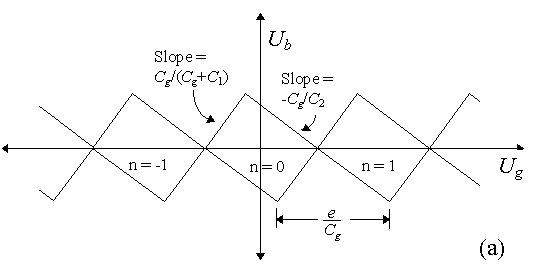
\includegraphics[width=250px]{Images/Diamant_Coulomb_Theorie.png}
        \caption{Diamant de Coulomb théorique}
        \label{fig:}
    \end{center}
\end{figure}

Quand on est à l'intérieur d'un de ces diamants, nous ne pouvons plus faire circuler d'électrons dans l'îlot. Quand nous sommes au-dessus ou en dessous d'un de ces diamants, il y a possibilité de faire rentrer puis sortir un électron un par un.

Il y a ainsi des pics de conductance pour certaines valeurs de tension de grille lorsque la dégénérescence entre les états de charges N et N+1 est atteinte. On appelle ces pics, pics de Coulomb.

Notre molécule unique de fullerène peut effectivement être considérée comme un point quantique, de par sa géométrie et sa taille. En effet elle est d'une taille de l'ordre d'un nanomètre, taille comparable à la longueur d'onde de Fermi ; il est donc raisonnable de penser que les électrons sont localisés dans les trois dimensions de l'espace.
